% \chapter{METODOLOGIA}
% \label{metodologia}
%--------------------------------------------------------------
\chapter{\textbf{EQUAÇÕES DE GOVERNO}}
\label{sec_eq_governo}
%--------------------------------------------------------------
\section{\textbf{Introdução}}
Este trabalho apresenta a modelagem de fluidos e partículas em um sistema de escoamento multifásico, portanto é preciso definir o que é um escoamento e quais as suas restrições para este trabalho.
Um escoamento é o movimento das moléculas de um fluido em conjunto.
As moléculas são tomadas como elementos infinitesimais, porém tratados de forma que não haja espaços vazios entre elas.
Isto permite que as propriedades do fluido sejam tratadas pontualmente, podendo variar por exemplo sua densidade ou velocidade de nó a nó.
Pode-se então modelar o comportamento destes escoamentos seguindo as equções de conservação:
\begin{itemize}
	\item \hyperref[cons_massa]{Conservação de Massa}
	\item \hyperref[cons_qmov]{Conservação de Quantidade de Movimento}
\end{itemize}

%--------------------------------------------------------------
\section{\textbf{Conservação de Massa}}
\label{sec_cons_massa}
O princípio de conservação de massa sem geração descreve que, dentro de um volume de controle, a soma da \textbf{taxa de acúmulo de massa dentro do volume} com \textbf{o fluxo de massa que atravessa a fronteira do volume} é nula como demonstrado por Pontes e Norberto (2010)\cite{pontes_norberto}.

O acúmulo de massa dentro do volume de controle é definido como:
\begin{equation}
    \int_{V_c}\dfrac{\partial}{\partial t} dm =  \int_{V_c}\dfrac{\partial}{\partial t} (\rho_f d V_c)
    \label{acumulo_massa}
\end{equation}
\begin{equation}
    m =  \rho_f V_c
    \label{densidade}
\end{equation}
onde $V_c$ é o volume de controle, $dm$ é o elemento infinitesimal de massa e $\rho_f$ é a massa específica do fluido.

Simplificando a equação de acúmulo de massa \eqref{acumulo_massa}, tomada para um volume de controle permanente, que não varia no tempo, tem-se:
\begin{equation}
    \int_{V_c}\dfrac{\partial}{\partial t} (\rho_f d V_c) = \int_{V_c}\dfrac{\partial \rho_f}{\partial t} d V_c + \int_{V_c} \rho_f \dfrac{\partial d V_c}{\partial t} = \int_{V_c}\dfrac{\partial \rho_f}{\partial t} d V_c
    \label{acumulo_massa_simp}
\end{equation}

E o fluxo de massa que atravessa a fronteira é retratado como:
\begin{equation}
    \oint_{S}\rho_f \vec{v}_f.\vec{n} dA
    \label{fluxo_massa}
\end{equation}
onde $S$ é a curva de contorno da fronteira do volume de controle, $\vec{v}_f$ é o campo de velocidades do fluido, $dA$ é o elemento infinitesimal de área da superfície de contorno do volume de controle e $\vec{n}$ é um vetor normal unitário orientado para fora do contorno $S$.

A conservação de massa é então representada como:
\begin{equation}
    \int_{V_c}\dfrac{\partial \rho_f}{\partial t} d V_c + \oint_{S}\rho_f \vec{v}_f.\vec{n} dA = 0
    \label{cons_mass}
\end{equation}

Pode-se rescrever a equação de conservação de massa aplicando-se o \textit{Teorema de Gauss}, apresentado por Pontes e Norberto (2010)\cite{pontes_norberto}, na integral de superfície:
\begin{equation}
    \int_{V_c}\dfrac{\partial \rho_f}{\partial t} d V_c + \int_{V_c}\vec{\nabla}.(\rho_f \vec{v}_f) d V_c = 
    \int_{V_c}\left(\dfrac{\partial \rho_f}{\partial t} + \vec{\nabla}.(\rho_f \vec{v}_f) \right)d V_c = 0
    \label{cons_mass_int}
\end{equation}
obtendo-se a equação integral da conservação de massa, onde $\vec{\nabla}$ é o operador diferencial gradiente de componentes $\vec{\nabla}=\left(\tfrac{\partial}{\partial \hat{i}}, \tfrac{\partial}{\partial \hat{j}}, \tfrac{\partial}{\partial \hat{k}}\right)$..

Ao considerar a conservação do ponto de vista local, pode-se remover o termo integral e escrever a forma diferencial da conservação de massa:
\begin{equation}
    \dfrac{\partial \rho_f}{\partial t} + \vec{\nabla}.(\rho_f \vec{v}_f) = 0
    \label{cons_mass_dif}
\end{equation}

Esta equação é denominada \textit{Equação da Continuidade}, e pode ser reescrita como:
\begin{equation}
    \dfrac{\partial \rho_f}{\partial t} + \vec{v}_f.\vec{\nabla} \rho_f + \rho_f \vec{\nabla}.\vec{v}_f = 0
    \label{continuity}
\end{equation}

Tomando-se algumas hipósteses, é possível simplificar mais a equação.
Para um fluido incompressível, com massa específica invariante na posição e no tempo, a equação da continuidade pode ser escrita como:
\begin{equation}
    \rho_f \vec{\nabla}.\vec{v}_f = 0
    \label{continuity_mid}
\end{equation}

Como a massa específica do fluido não pode ser nula, tem-se:
\begin{equation}
    \vec{\nabla}.\vec{v}_f = 0
    \label{continuity_final}
\end{equation}
tomada para um \textbf{fluido incompressível}.


%--------------------------------------------------------------
\section{\textbf{Conservação de Quantidade de Movimento}}
\label{sec_cons_qmov}
A conservação de quantidade de movimento é similar a conservação de massa, porém é tomada como um termo vetorial.
Para o caso deste trabalho, é utilizada a versão linear da conservação de quantidade de movimento.
Portanto, tem-se que a conservação da quantidade de movimento determina que a \textbf{taxa de acúmulo de quantidade de movimento linear dentro do volume de controle} mais \textbf{o fluxo de quantidade de movimento linear que atravessa a fronteira do volume de controle} é igual a \textbf{soma das forças aplicadas à superficie da fronteira do volume de controle e as forças do volume}.

A definição da taxa de acúmulo de quantidade de movimento linear dentro do volume de controle é:
\begin{equation}
    \int_{V_c}\dfrac{\partial}{\partial t} (\rho_f \vec{v}_f) d V_c
    \label{acumulo_qmov}
\end{equation}

E o fluxo de quantidade de movimento que atravessa a fronteira é retratado como:
\begin{equation}
    \oint_{S}\rho_f \vec{v}_f \vec{v}_f.\vec{n} dA
    \label{fluxo_qmov}
\end{equation}

As forças aplicadas à superfície da fronteira do volume de controle é:
\begin{equation}
    \oint_{S}\boldsymbol{\sigma}.\vec{n} dA
    \label{result_sup_qmov}
\end{equation}
onde $\boldsymbol{\sigma}$ é o tensor de tensões.

E as forças de volume são, tomada apenas a força gravitacional:
\begin{equation}
    \int_{V_c}\rho_f \vec{g} dV_c
    \label{result_vol_qmov}
\end{equation}
onde $\vec{g}$ é a aceleração gravitacional presente.

Montando-se a equação, a conservação de quantidade de movimento é representada como:
\begin{equation}
    \int_{V_c}\dfrac{\partial}{\partial t} (\rho_f \vec{v}_f) d V_c + 
    \oint_{S}\rho_f \vec{v}_f \vec{v}_f.\vec{n} dA =
    \oint_{S}\boldsymbol{\sigma}.\vec{n} dA +
    \int_{V_c}\rho_f \vec{g} dV_c
    \label{cons_qmov}
\end{equation}

Novamente, aplica-se o \textit{Teorema de Gauss} nas integrais de superfície e extrai-se a forma integral da equação da conservação de quantidade de movimento:
\begin{equation}
    \int_{V_c}\dfrac{\partial}{\partial t} (\rho_f \vec{v}_f) d V_c + 
    \int_{V_c}\vec{\nabla}.(\rho_f \vec{v}_f.\vec{v}_f) dV_c =
    \int_{V_c}\vec{\nabla}.\boldsymbol{\sigma} dV_c +
    \int_{V_c}\rho_f \vec{g} dV_c
\end{equation}

Simplificando:
\begin{equation}
    \int_{V_c} \left(
	    \dfrac{\partial}{\partial t} (\rho_f \vec{v}_f) + 
	    \vec{\nabla}.(\rho_f \vec{v}_f.\vec{v}_f) -
	    \vec{\nabla}.\boldsymbol{\sigma} -
	    \rho_f \vec{g}
    \right) = 0
    \label{cons_qmov_int}
\end{equation}

Novamente, considerando-se a conservação do ponto de vista pontual, remove-se o termo integral para escrever a forma diferencial da conservação de quantidade de movimento:
\begin{equation}
    \dfrac{\partial}{\partial t} (\rho_f \vec{v}_f) + 
    \vec{\nabla}.(\rho_f \vec{v}_f.\vec{v}_f) =
    \vec{\nabla}.\boldsymbol{\sigma} +
    \rho_f \vec{g}
    \label{cons_qmov_dif}
\end{equation}

Continuando a desenvolver a equação:
\begin{equation}
    \dfrac{\partial}{\partial t} (\rho_f \vec{v}_f) + 
    \vec{\nabla}(\rho_f \vec{v}_f.\vec{v}_f) =
    \rho_f \dfrac{\partial \vec{v}_f}{\partial t} + 
    \vec{v}_f \dfrac{\partial \rho_f}{\partial t} + 
    \rho_f \vec{v}_f.\vec{\nabla}.\vec{v}_f +
    \vec{v}_f.\vec{\nabla}.(\rho_f \vec{v}_f)
    \label{cons_qmov_ini}
\end{equation}
\begin{equation}
    \rho_f \left(
    	\dfrac{\partial \vec{v}_f}{\partial t} +
    	\vec{v}_f.\vec{\nabla}.\vec{v}_f 
	\right) +
	\vec{v}_f \left(
    	\dfrac{\partial \rho_f}{\partial t} +
    	\vec{\nabla}.(\rho_f \vec{v}_f)
	\right)
    \label{cons_qmov_mid}
\end{equation}

Novamente, é tomanda a hipóstese de um fluido incompressível.
Portanto, a equação pode ser simplificada para ser escrita como:
\begin{equation}
    \rho_f \left(
    	\dfrac{\partial \vec{v}_f}{\partial t} + 
    	\vec{v}_f.\vec{\nabla}.\vec{v}_f
	\right) =
    \vec{\nabla}.\boldsymbol{\sigma} +
    \rho_f \vec{g}
    \label{cons_qmov_fin}
\end{equation}

Reescrevendo o tensor de tensões como uma soma de dois tensores, e o substituindo na equação, tem-se:
\begin{equation}
    \boldsymbol{\sigma} = -p\mathbf{I} + \boldsymbol{\tau}
    \label{sigma}
\end{equation}
\begin{equation}
    \rho_f \left(
    	\dfrac{\partial \vec{v}_f}{\partial t} + 
    	\vec{v}_f.\vec{\nabla}.\vec{v}_f
	\right) =
    -\vec{\nabla}p +
    \vec{\nabla}.\boldsymbol{\tau} +
    \rho_f \vec{g}
    \label{cons_qmov_tensor}
\end{equation}
onde p é o campo de pressões no fluido, $\mathbf{I}$ é a matriz de indentidade e $\boldsymbol{\tau}$ é o tensor de tensões viscosas.

Novamente é necessário fazer uma hipótese para este escoamento, para que seja possível definir as forças atuantes no fluido. 
O tensor de tensões viscosas $\boldsymbol{\tau}$ está relacionado as propriedades do fluido, podendo ser definido matematicamente para um fluido homogêneo, isotrópico e newtoniano, como:
\begin{equation}
    \boldsymbol{\tau} = \mu_f\left(\vec{\nabla}.\vec{v}_f + \left(\vec{\nabla}.\vec{v}_f \right)^T \right)
    \label{tau}
\end{equation}
onde $\mu_f$ é a viscosidade dinâmica do fluido.

Substituindo a definição de $\boldsymbol{\tau}$ na \refeq{cons_qmov_tensor}, obtem-se:
\begin{equation}
    \rho_f \left(
    	\dfrac{\partial \vec{v}_f}{\partial t} + 
    	\vec{v}_f.\vec{\nabla}.\vec{v}_f
	\right) =
    -\vec{\nabla}p +
    \vec{\nabla}.\left(\mu_f\left(\vec{\nabla}.\vec{v}_f + \left(\vec{\nabla}.\vec{v}_f \right)^T \right)\right) +
    \rho_f \vec{g}
\end{equation}

Assumindo-se que a viscosidade dinâmica é constante para todo o fluido:
\begin{equation}
    \rho_f \left(
    	\dfrac{\partial \vec{v}_f}{\partial t} + 
    	\vec{v}_f.\vec{\nabla}.\vec{v}_f
	\right) =
    -\vec{\nabla}p +
    \mu_f \vec{\nabla}.\left(\vec{\nabla}.\vec{v}_f + \left(\vec{\nabla}.\vec{v}_f \right)^T \right) +
    \rho_f \vec{g}
\end{equation}
\begin{equation}
    \rho_f \left(
    	\dfrac{\partial \vec{v}_f}{\partial t} + 
    	\vec{v}_f.\vec{\nabla}.\vec{v}_f
	\right) =
    -\vec{\nabla}p +
    \mu_f \left(\nabla^2\vec{v}_f + \vec{\nabla}.\left(\vec{\nabla}.\vec{v}_f \right)^T \right) +
    \rho_f \vec{g}
    \label{tau_last}
\end{equation}

Utilizando o que foi obtido na Equação de Continuidade \refeq{continuity_final} pode-se substituir na equação \refeq{tau_last}:
\begin{equation}
    \rho_f \left(
    	\dfrac{\partial \vec{v}_f}{\partial t} + 
    	\vec{v}_f.\vec{\nabla}.\vec{v}_f
	\right) =
    -\vec{\nabla}p +
    \mu_f \nabla^2\vec{v}_f +
    \rho_f \vec{g}
    \label{tau_simple}
\end{equation}

Dividindo-se todos os termos pela massa específica pode-se reescrever a equação \refeq{tau_simple}, obtem-se então a forma simplificada da \textit{Equação de Navier-Stoakes} para fluidos neutonianos incompressíveis e com viscosidade constante:
\begin{equation}
	\dfrac{\partial \vec{v}_f}{\partial t} + 
	\vec{v}_f.\vec{\nabla}.\vec{v}_f =
    -\dfrac{1}{\rho_f} \vec{\nabla}p +
    \dfrac{\mu_f}{\rho_f} \nabla^2\vec{v}_f +
    \vec{g}
    \label{navier}
\end{equation}

%--------------------------------------------------------------
\section{\textbf{Formulação Corrente-Vorticidade}}
\label{sec_corr_vort}
A formulação de corrente-vorticidade é um sistema de equações que providencia um método alternativo de se calcular as propriedades de um escoamento sem solucionar diretamente a equação de Navier-Stoakes \eqref{navier}.
Isto permite simplificar a solução do problema, pois a Equação de Navier-Stoakes possui um forte acoplamento entre o campo de pressões e o campo de velocidades.

Para isso, é utilizada a seguinte identidade vetorial:
\begin{equation}
    \vec{v}.\vec{\nabla}.\vec{v} = \vec{\nabla} \dfrac{v^2}{2} - \vec{v}\times\vec{\nabla}\times\vec{v}
    \label{ident_vetor} 
\end{equation}

Substituindo na \refeq{navier}:
\begin{equation}
	\dfrac{\partial \vec{v}_f}{\partial t} + 
	\vec{\nabla} \dfrac{v^2_f}{2} -
	\vec{v}_f\times\vec{\nabla}\times\vec{v}_f =
    -\dfrac{1}{\rho_f} \vec{\nabla}p +
    \dfrac{\mu_f}{\rho_f} \nabla^2\vec{v}_f +
    \vec{g}
\end{equation}

Em seguida, aplica-se o operador rotacional nos dois lados da equação:
\begin{equation}
	\vec{\nabla}\times\dfrac{\partial \vec{v}_f}{\partial t} + 
	\vec{\nabla}\times\vec{\nabla} \dfrac{v^2_f}{2} -
	\vec{\nabla}\times\vec{v}_f\times\vec{\nabla}\times\vec{v}_f =
    -\vec{\nabla}\times\dfrac{1}{\rho_f} \vec{\nabla}p +
    \vec{\nabla}\times\dfrac{\mu_f}{\rho_f} \nabla^2\vec{v}_f +
    \vec{\nabla}\times\vec{g}
\end{equation}

Simplifica-se então a equação, pois os termos que possuem o operador gradiente são anulados, pois o rotacional do gradiente de um escalar é zero.
O termo gravitacional também é anulado já que a derivada da constante $\vec{g}$ é zero.
Fica-se com a seguinte equação:
\begin{equation}
	\dfrac{\partial}{\partial t}(\vec{\nabla}\times\vec{v}_f)-
	\vec{\nabla}\times\vec{v}_f\times\vec{\nabla}\times\vec{v}_f =
    \dfrac{\mu_f}{\rho_f} \nabla^2 (\vec{\nabla}\times\vec{v}_f)
\end{equation}

Define-se o vetor $\vec{\omega}$ como \textit{vorticidade}, onde $\vec{\omega}=\vec{\nabla}\times\vec{v}_f$.
Substitui-se na equação:
\begin{equation}
	\dfrac{\partial \vec{\omega}}{\partial t} -
	\vec{\nabla}\times\vec{v}_f\times\vec{\omega} =
    \dfrac{\mu_f}{\rho_f} \nabla^2 \vec{\omega}
\end{equation}

Rearranjando-se as operações vetoriais, tem-se:
\begin{equation}
	\dfrac{\partial \vec{\omega}}{\partial t} +
	\vec{v}_f.\vec{\nabla}.\vec{\omega} -
	\vec{\omega}.\vec{\nabla}.\vec{v}_f =
    \dfrac{\mu_f}{\rho_f} \nabla^2 \vec{\omega}
\end{equation}

Como a vorticidade é perpendicular ao vetor velocidade, para escoamentos bidimensionais pode-se anular o produto $\vec{\omega}.\vec{\nabla}.\vec{v}_f$ como demonstrado por Pontes e Norberto (2010)\cite{pontes_norberto}.
Então obtem-se a \textit{Equação da Vorticidade} para escoamentos de fluidos neutonianos incompressíveis:
\begin{equation}
	\dfrac{\partial \vec{\omega}}{\partial t} +
	\vec{v}_f.\vec{\nabla}.\vec{\omega} =
    \dfrac{\mu_f}{\rho_f} \nabla^2 \vec{\omega}
    \label{vorticity}
\end{equation}

Para escoamentos permanentes bidimensionais de fluidos incompressíveis, a velocidade é calculada pela vazão volumétrica.
Portanto, a velocidade pode ser substituída por um escalar $\psi$, conhecido como \textit{função corrente}.
A relação entre a função corrente e o campo de velocidades do fluido é obtida através da manipulação da equação da continuidade \eqref{continuity}, dada como:
\begin{equation}
	\dfrac{\partial v_x}{\partial x} +
	\dfrac{\partial v_y}{\partial y} =
	0
\end{equation}
onde $v_x$ é a componente do campo de velocidades do fluido no eixo $x$ e $v_y$ é a componente do campo de velocidades do fluido no eixo $y$.

E a relação entre elas é apresentada em seguida:
\begin{equation}
	v_x = \dfrac{\partial \psi}{\partial y}
	\label{corr_x}
\end{equation}
\begin{equation}
	v_y = -\dfrac{\partial \psi}{\partial x}
	\label{corr_y}
\end{equation}

Enquanto a relação entre a função corrente e a vorticidade é:
\begin{equation}
	(\vec{\nabla}\times\vec{v}_f)_z =
	\dfrac{\partial v_y}{\partial x} -
	\dfrac{\partial v_x}{\partial y}
\end{equation}

Substituindo os termos de velocidade pelas equações \refeq{corr_x} e \refeq{corr_y}:
\begin{equation}
	\omega_z =
	-\dfrac{\partial}{\partial x}\dfrac{\partial \psi}{\partial x} -
	\dfrac{\partial}{\partial y}\dfrac{\partial \psi}{\partial y}
\end{equation}
\begin{equation}
	\omega_z =
	-\nabla^2\psi
	\label{corrente_vorticidade}
\end{equation}

Então o sistema de corrente-vorticidade é apresentado como:
\begin{equation}
	\dfrac{\partial \vec{\omega}}{\partial t} +
	\vec{v}_f.\vec{\nabla}.\vec{\omega} =
    \dfrac{\mu_f}{\rho_f} \nabla^2 \vec{\omega}
    \label{fluid_eq1}
\end{equation}
\begin{equation}
	\nabla^2\psi =
	-\omega_z
    \label{fluid_eq2}
\end{equation}
\begin{equation}
	\vec{v}_f = \left(\dfrac{\partial \psi}{\partial y},
	-\dfrac{\partial \psi}{\partial x} \right)
    \label{fluid_eq3}
\end{equation}


%--------------------------------------------------------------
\section{\textbf{Número de Reynolds}}
\label{sec_reynolds}
Para analisar as características de escoamentos com diversas variáveis, utiliza-se $Re$, uma constante adimensional conhecida como \textbf{Número de Reynolds}.

O número de Reynolds permite reconhecer rapidamente as qualidades de um escoamento apenas por seu valor.
Ele estabelece uma relação entre as forças viscosas e inerciais de um fluido.
Pode-se delcarar então qual força possui maior componente no comportamento do escoamento.

O número de Reynolds de um escoamento é calculado por:
\begin{equation}
    Re = \dfrac{\rho_f |\vec{v}_{f}|_{max} D}{\mu_f} 
    \label{reynolds}
\end{equation}
onde $v_{fmax}$ é a maior velocidade do campo de velocidades do fluido, e $D$ é o comprimento característico de problema.


%--------------------------------------------------------------
\section{\textbf{Forças Exercidas em Partículas}}
\label{sec_eq_part}
A principal equação que governa o comportamento do movimento das partículas é obtida a partir da 2ª Lei de Newton como demonstrado por Crowe et al. (2011)\cite{crowe}.
\begin{equation}
    \sum\vec{F}_{p} = \dfrac{d(m_p\vec{v}_p)}{dt}
    \label{newton} 
\end{equation}
onde $\sum\vec{F}_{p}$ é o somatório de forças aplicadas a partícula, $m_p$ é a massa e $\vec{v}_p$ a velocidade da partícula.

As forças aplicadas às partículas foram determinadas a partir da equação de \textbf{Basset–Boussinesq–Oseen} (BBO), que descreve as forças sofridas por partículas sob efeito de escoamentos com número de Reynolds \ref{sec_reynolds} pequeno.
Porém, o número de Reynolds utilizados é diferente do calculado para escoamentos, utiliza-se um valor específico para cada partícula.
\begin{equation}
    Re_{p} = \dfrac{\rho_p |\left(\vec{v}_{f} - \vec{v}_{p} \right)|_{max} d_{p}}{\mu_f}
    \label{reynolds_p}
\end{equation}
onde $\rho_p$ é a densidade, $d_p$ o diâmetro e $\vec{v}_{p}$ a velocidade da partícula, e $\vec{v}_{f}$ é a velocidade do escoamento na mesma posição da partícula.

Como mencionado, as forças da equação de BBO representam fielmente o comportamento real de partículas para valores de Reynolds menores que $1$,  ou seja, $Re_{p} < 1$.

Nem todas as forças apresentadas na equação BBO foram inseridas no código de simulação.
Elas foram inseridas sequencialmente durante o desenvolvimento do código, seguidas de testes para verificar sua implementação.
Foram escolhidas apenas as principais forças, apresentadas a seguir, por Crowe et al. (2011)\cite{crowe}: 
\begin{itemize}
    \item \textbf{Força Gravitacional}:
        Também conhecida como força Peso, criada pelo campo graviacional do planeta aplicado aos corpos com massa.
        Seu valor é calculado através das massas dos corpos, a distância entre seus centros de massa e uma constante universal.
        Porém, para simplificar o problema, pode-se assumir que a distância entre eles é constante e igual ao raio do planeta Terra.
        Portanto, pode-se assumir que o valor da força será sempre constante e proporcional a uma aceleração constante aplicada a massa da partícula, o que torna esta a força mais simples de se calcular:
        \begin{equation}
            \vec{F}_{grav} = m_p \vec{g}
            \label{grav}
        \end{equation}
        onde $\vec{g}$ é tomada como a aceleração constante da gravidade na superfície terrestre com valor definido de $\vec{g} = (0, -9.80665)m/s^2$.

    \item \textbf{Força de Arrasto}:
        Força causada pelo atrito do fluido no contorno da partícula, que cria um efeito cisalhante e tende deixar a partícula com mesma velocidade que o fluido.

        Sua equação é determinada como:
        \begin{equation}
            \vec{F}_{drag} = 3 \pi \mu_f d_p \left(\vec{v}_{f} - \vec{v}_{p} \right)
            \label{drag}
        \end{equation}

        Pode-se observar seu comportamento presente no termo de velocidade relativa $\left(\vec{v}_{f} - \vec{v}_{p} \right)$ da equação \refeq{drag}.
        Este termo causa o efeito de aproximar a velocidade da partícula à velocidade do fluido já que torna a força proporcionalmente maior quanto mais afastadas elas se encontrarem.
        E o sinal permite que caso a partícula esteja mais rápida ela seja desacelerada e o inverso se ela se encontrar mais lenta. 

    \item \textbf{Força de Sustentação}:
        A força de sustentação é uma componente que tende a mover a partícula em direções perpendiculares a seu movimento principal.
        Ela possui várias formas de ser calculada, sendo nomeada para cada caso.

        Por exemplo, a \textbf{Força de Magnus} está relacionada a rotação, ou velocidade angular, presente na partícula.
        Neste trabalho as partículas são assumidas como corpos rígidos sem rotação, então está força não será levada em conta.

        Porém outro tipo de força de sustentação é a \textbf{Força de Saffman} explorada por Crowe et al. (2011)\cite{crowe}, que é gerada a partir do gradiente de velocidades presente no escoamento.
        Para que haja o efeito da força de sustentação de Saffman é necessário que exista um gradiente no campo de velocidades diferente de nulo, como pode se notar na \ref{saffman}.
        \begin{figure}[H]
            \centering
            \stackunder{
                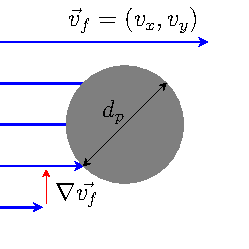
\includegraphics[width=0.5\linewidth]{figures/saffman_lift.pdf}
            } {\raggedleft \scriptsize Fonte: Autor.}
            \caption{Partícula em um escoamento com um gradiente de velocidade não nulo.}
            \label{saffman}
        \end{figure}

        A força é aplicada em uma direção perpendicular ao movimento do escoamento e proporcional ao crescimento da velocidade no escoamento.
        Ela pode ser calculada através da equação:
        \begin{equation}
            \vec{F}_{lift} = 1.61 \mu_f d_p \left(\vec{v}_{f} - \vec{v}_{p} \right) \sqrt{{Re}_G}
            \label{lift}
        \end{equation}
        onde $Re_{G}$ é conhecido como número de Reynolds de cisalhamento, e é calculado através da equação:
        \begin{equation}
            Re_G = \dfrac{d_p^2 \rho_f}{\mu_f} \nabla \vec{v}_f
            \label{reg}
        \end{equation}

    \item \textbf{Força de Massa Virtual} \textit{(Added Mass)}:
        A força de massa virtual está relacionada ao trabalho realizado pelo fluido para acelerar um corpo submerso.
        Isto pode ser interpretado como a energia que seria utilizada para mover uma mesma quantidade de fluido no lugar do corpo presente.
        O valor desta força pode ser calculado através da equação:
        \begin{equation}
            \vec{F}_{mass} = \dfrac{1}{2} \rho_f V_p \dfrac{d}{dt}\left(\vec{v}_{f} - \vec{v}_{p} \right)
            \label{mass}
        \end{equation}
        onde $V_p$ é o volume da partícula inserida no escoamento.
\end{itemize}